\documentclass[a4paper,12pt]{IEEEtran}
\usepackage{graphicx}
\graphicspath{{./report_plots/}}
\begin{document}

\title{CSC 510 Assignment 1 Report}
\author{Justin Oakley}
\maketitle

\pagenumbering{arabic}
\tableofcontents
\newpage

\section{Introduction}
This report is about knowing and preparing given data in order to understand its characteristics. It also features a summary of a paper on the problems and challenges of machine learning in big data classification. The reason that these analyses are important to go through is that it will assist in developing skills that are needed in the field of data science and big data. Such attributes that necessary in this field of study are understandings of the importance of data, systems, machine learning techniques, scalability and complexity as well as big data systems and programming languages that are most commonly associated with said systems. In this assignment, four different data files were used for analyzation, \textit{carpet.csv, hardwood.csv, bgg\_db\_2017\_04.csv}, and \textit{bgg\_db\_2018\_01.csv}, via the Python 3 language (using libraries such as Pandas and Matplotlib) and its respective version of the Apache Spark technology. All of these were a gateway for an in-depth and readable analysis on fundamental processes used in big data science, and a greater knowledge of how technologies such as Apache Spark function.

\section{Carpet and Hardwood Datasets}
The following datasets used in the first portion of this analysis are called \textit{Carpet Floor} and \textit{Hardwood Floor}, and are computationally derived from the following .jpeg files. Both of these datasets individually contain one thousand twenty-four observations and sixty-four feature columns where each feature observation is a numerical value. Knowing this, all sixty-four features per dataset are processed for statistical information, then utilized for the steps of data visualization. Immediately following these parts, both datasets are labeled based on which file each observation originates from, then is merged and randomized and finally split into two different sets, the training and testing sets.

\subsection{Statistical Information}
\label{sec1}
Using basic statistical analysis on the first and last feature columns in the \textit{Carpet Floor} dataset, '\_c0' and '\_c63', it was observed that both features have means of approximately 99.29 and 98.92 and standard deviations of approximately 17.92 and 18.38. Now, when the covariance and the correlation of both features are calculated, it results in approximately 75.79 and 0.15. With this information in mind, it was determined that both carpet features have zero linear correlation between the two of them, though that does not mean that there is not a relationship with these features. The first and last features of \textit{Hardwood Floor} dataset, on the otherhand, have means of 99.29 and 98.92 and standard deviations of 17.92 and 18.38, as well as a sample covariance of about 225.00 and a correlation of 0.68. Having this knowledge in mind, it was then determined that while the carpet and hardwood datasets do not have linearly correlating features, their features share some type of a relationship between each other because both sets have almost equivalent means and standard deviations.

\subsection{Data Visualization}
\label{sec2}
The following images are graphic visualizations of the overall mean and standard deviation values in relation to the incrementally increasing number of features for both the carpet and hardwood datasets. While the values in each respective graph tend to have a visually distinct change with each addition of a feature, they never seem to radically change. In fact, the averages and variances of only one feature and sixty-four features for the carpet dataset are have similar numerical values, while the averages of only one feature and sixty-four features for the hardwood dataset are approximately equivalent but the variance seems to increase with an increase in features. What this means is that the observations within the carpet dataset are similar despite the growing number of features while hardwood dataset observations increasingly differ with the inclusion of more features.
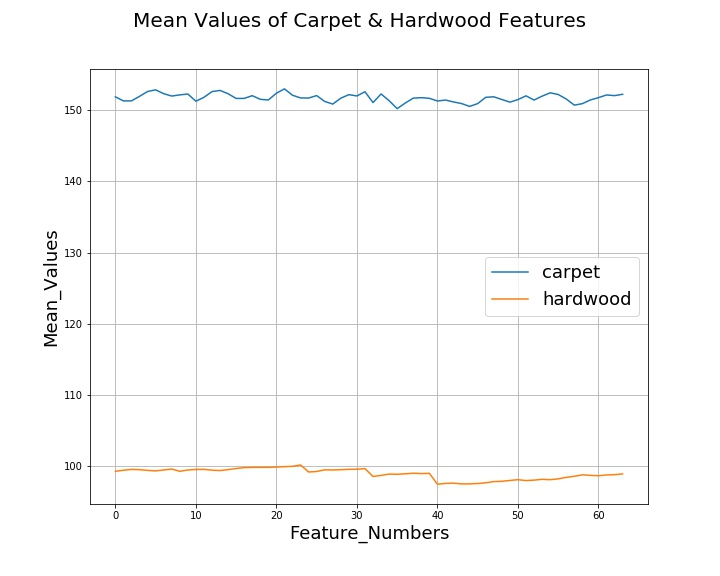
\includegraphics[width=8cm]{carpethardwood_mean}
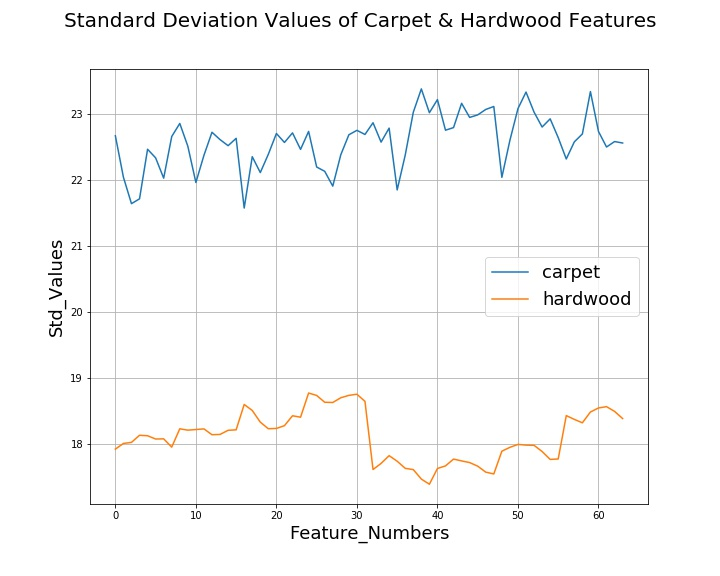
\includegraphics[width=8cm]{carpethardwood_stddev}
According to the two histograms created from the first feature of the carpet and hardwood observations, both sets apparently follow Gaussian distributions. By using this knowledge, detecting skewness in the data will be less complex to perform. This also means that any proababilistic and statistical methods applied to either datasets will result in patterns following a bell-shaped curve.
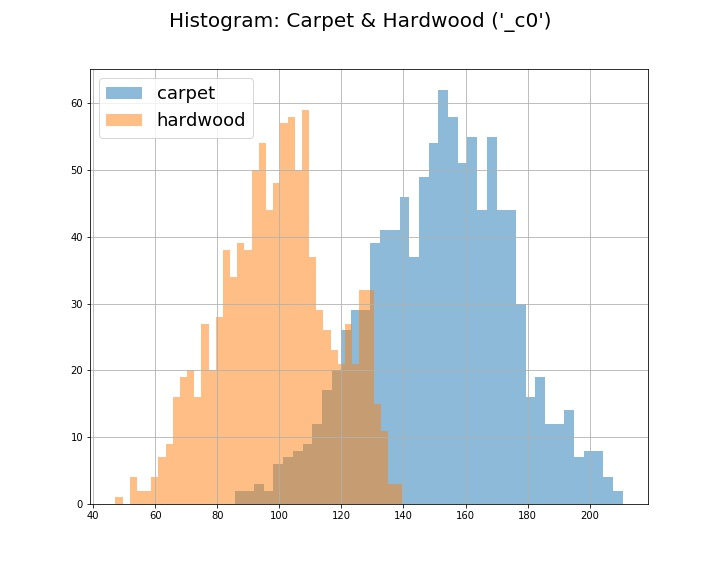
\includegraphics[width=8cm]{carpethardwood_hist01}

\subsection{Data Inference}
\label{sec3}
Now that statistical extraction and data visualization has been performed, characteristics of the data can be appropriately identified.
\begin{enumerate}
\item On the topic of data pattern deformation, neither the carpet nor hardwood datasets are imbalanced, inaccurate, or incomplete; all of which been observed in a three-dimensional scatter-plot composed of three features from each respective set.
\item Neither the carpet and hardwood datasets should be classified as big data for two reasons. (1) Both datasets have features that are the same data type, which means that it does not feature much variety. (2) The number of observations is far greater than the number of features in the carpet and hardwood datasets, meaning the data is not highly dimensional.
\item While normalization and standardization are not required for pattern detection for either of the two datasets, it is extremely helpful in data visualization because it allows the for comparing and contrasting carpet and hardwood data to be simplified. For example, the following images demonstrate that when plotting the first, fifty-fourth, and fifty-ninth features, it shows that the hardwood features will follow a more linear trend than the carpet features.
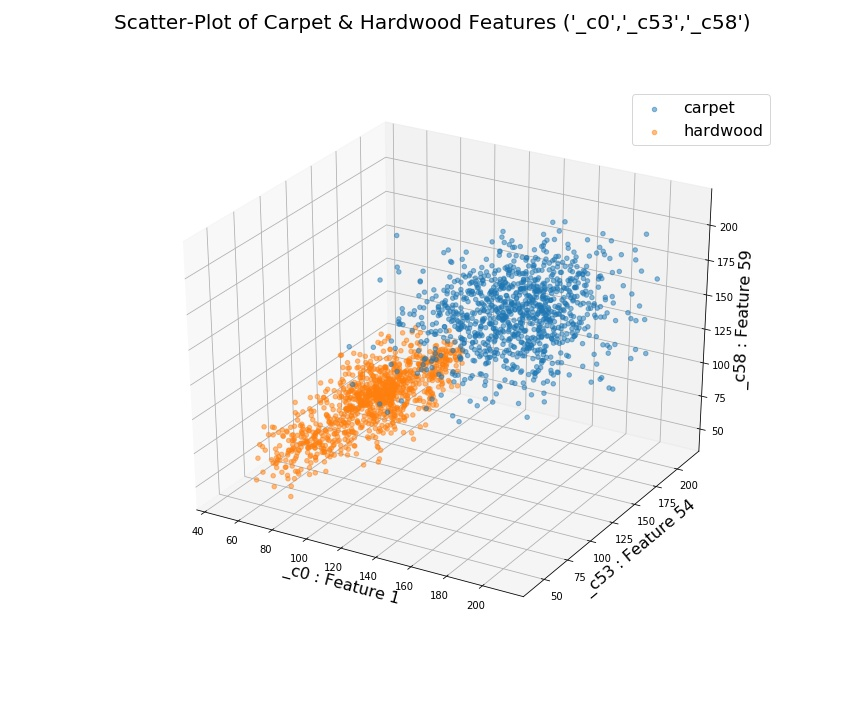
\includegraphics[width=8cm]{carpethardwood_3d01}
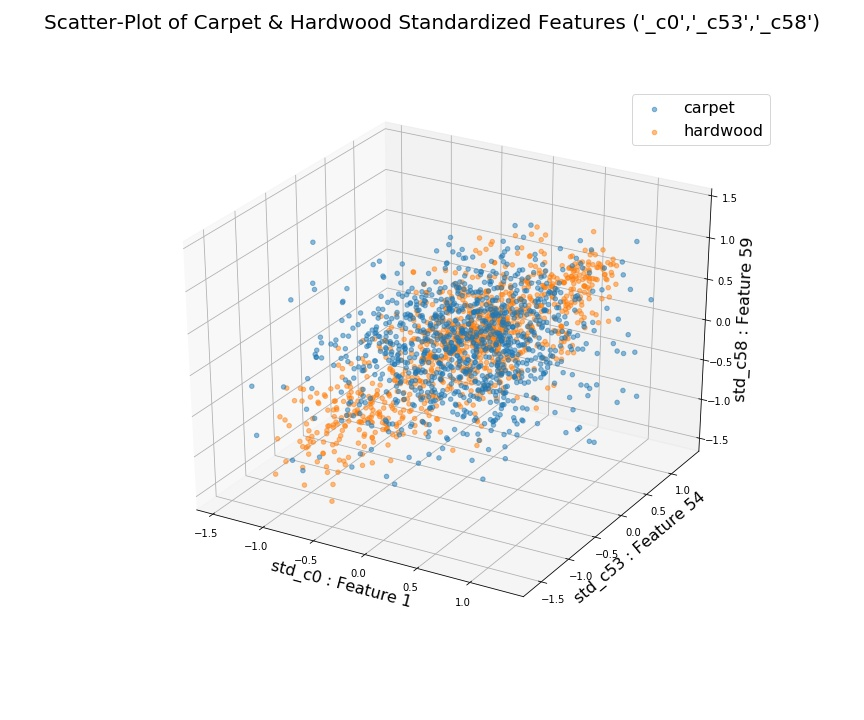
\includegraphics[width=8cm]{carpethardwood_3d02}
\end{enumerate}


\subsection{Constructing Training and Test Sets}
\label{sec4}
The construction of the training and testing sets from these two datasets is important because it allows for a greater understanding of the role of classification in big data science. For instance, when the carpet and hardwood datasets were originally given, they did not have labels which means attempting to classify the both sets in their initial states would prove difficult; but since both datasets where given individual labels so that carpet and hardwood observations could be distinguished and then merged together, this will make a way for a machine to undergo supervised learning. Also, when the data observations are randomized and split using an 80:20 ratio, it creates almost evenly balanced set between the training and testing test, which could possibly result in classifying or predicting data accuracy via machine learning techniques to be higher.

\section{Board Game Data From 2018 and 2019}
The following datasets utilized in this last portion of this report are called \textit{bgg\_db\_2017\_04.csv} and \textit{bgg\_db\_2018\_01.csv}. Both of these datasets are compiled of a variety of different commerical board games and come with features that both describe characteristics about game properties, approximate game length sessions, categories of ratings given to said game. There are a total of 4999 observations per dataset and only eleven numerical features are utilized for the following analysis process. This portion of the report will follow the same statistical information, data visualization and inference procedures as used in the \textit{Carpet Floor} and \textit{Hardwood Floor} sets.

\subsection{Statistical Information}
\label{sec5}
For the board game data basic statistical analysis, the features 'avg\_rating' and 'geek\_rating' were used in the computation process where 'avg\_rating' stands for the average rating of the board game and 'geek\_rating' is the rating given by the website, https://boardgamegeek.com/. The calculated mean of avg\_rating from the 2017 board game data and 2018 board game data were 6.93 and 6.06 while the mean of geek\_rating from 2017 and 2018 were 6.96 and 6.08. Meanwhile the calculated standard deviation of 2017's avg\_rating and geek\_rating are 0.57 and 0.48 and 2018's avg\_rating and geek\_rating are 0.56 and 0.48. Using this, the covariance of avg\_rating and geek\_rating from 2017 comes out to be 0.12 and the covariance of the 2018 counterparts is 0.13. This all leads to the correlation between these features for 2017 and 2018 to be 0.46 and 0.47, respectively. Thus, it is safe to assume that there is no linear correlation between avg\_rating and geek\_rating in either 2017 or 2018. Also, it can be seen that the statistical values of avg\_rating and geek\_rating had only a miniscule transformation in approximately one year's time.

\subsection{Data Visualization}
\label{sec6}
The following line graphs provide visual proof that the numerical features from the 2017 and 2018 board game data are similar in value to each other because both datasets have almost equivalent mean and variance values per number of included features.
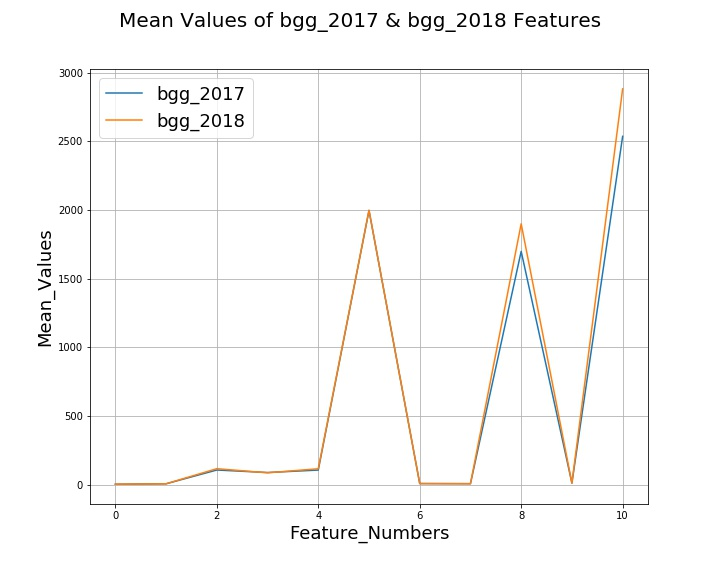
\includegraphics[width=8cm]{bgg_mean}
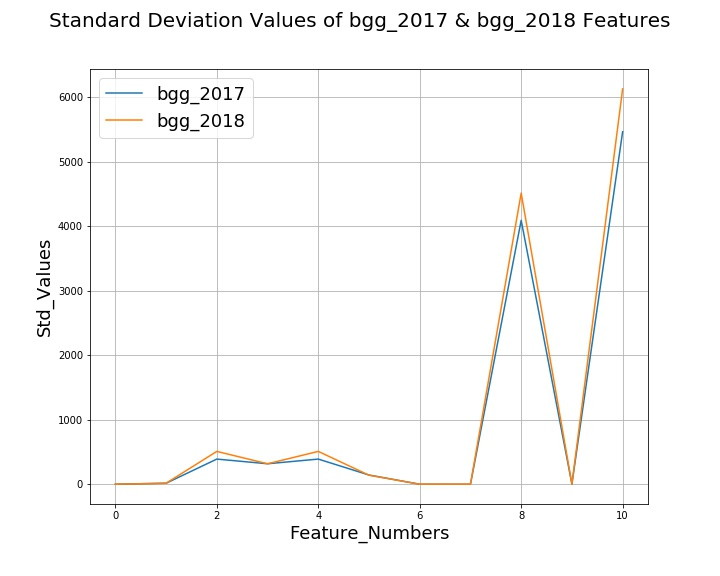
\includegraphics[width=8cm]{bgg_stddev}
As for the histograms below, they demonstrate that both board game datasets follow normal distributions in which the two distributions appear to be left-positively skewed. The skewness of the 2017 and 2018 patterns are good signs for classification since it will be easier to explain data characteristics.
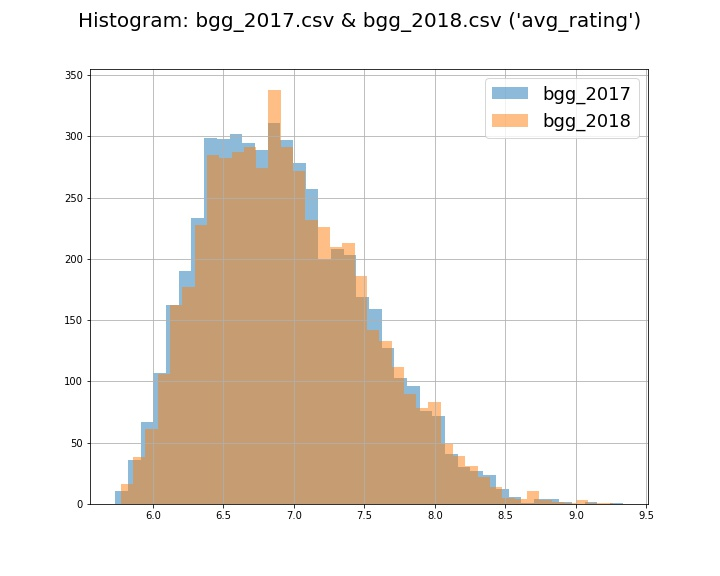
\includegraphics[width=8cm]{bgg_hist01}

\subsection{Data Inference}
\label{sec7}
With the basic statistical information extracted and both datasets have been plotted, the following characteristics of the 2017 and 2018 board game data were inferred.
\begin{enumerate}
\item Neither of the board game datasets appear to be suffering from any type of data deformation since they contain the same amount of observations and features, and each feature column did not appear to be containing any null values.
\item The data, once merged, could be considered big data, though low-dimensional, due to the fact that all feature columns were not of the same datatype (only the numerical values were utilized in previous computations and analysis) and the 2018 board game data set is an updated version of the data given in the 2017 game set.
\item Normalizing and standardizing the data, while grant some visual assistance to the datasets, is not need in the data processing since both graphs tend to retain the same bell-shaped pattern for each of their respective histograms and three-dimensional scatter-plots.
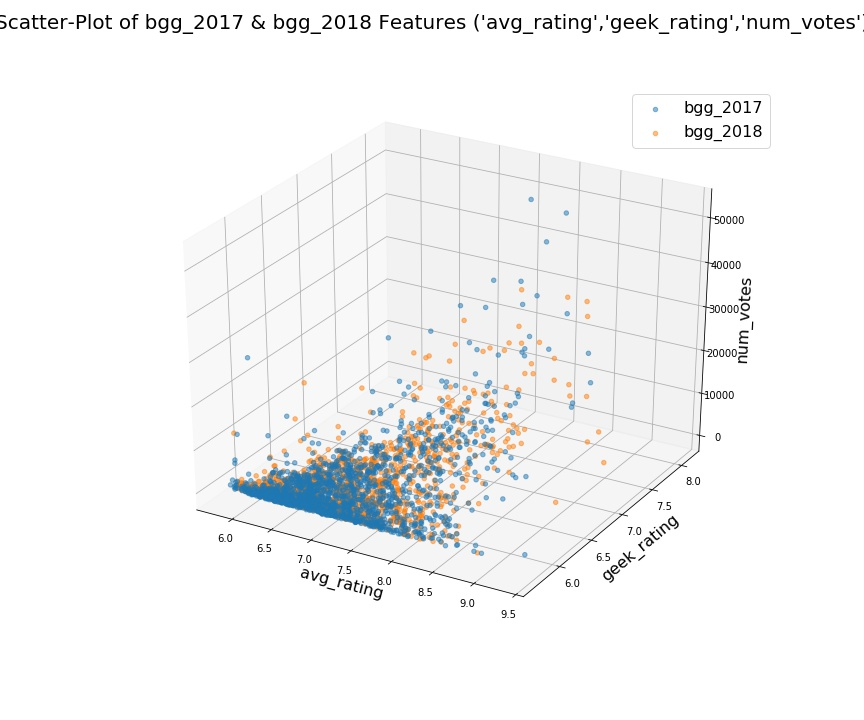
\includegraphics[width=8cm]{bgg_3d01}
\end{enumerate}

\section{Differences Between Floor and Board Game Data}
While the carpet and hardwood datasets and the board game datasets from 2017 and 2018 appear to have some similarities in terms of distribution patterns and statistical information, each dataset has major differences and comes with its own issues. The carpet and hardwood data cannot be classified as big data (Section \ref{sec1}, page \pageref{sec1}) while the board game data can be (Section \ref{sec7}, page \pageref{sec7}. Other issues that carpet and hardwood face is that unlike the board game data, these datasets cannot, individually, be classified due to a lack of labels included with the original data. On the other hand, the board game data from 2017 and 2018 are extremely similar in value to each other (Section \ref{sec5}, page \pageref{sec5} for more details) which can cause some visualization classification and pattern detection issues, if not careful, while the carpet and hardwood floor datasets are similar enough to make fair comparisons yet still be able to determine distinct differences in the floor data (Section \ref{sec2}, page \pageref{sec2}). Also, the number of features used in the combined carpet and hardwood floor data (Section \ref{sec4}, page \pageref{sec4}) will make it easier for machines to classify via supervised learning than the ones from board game data from 2017 and 2018 because the number of numerical features in the floor datasets is much larger than the board game dataset features.

\section{Summary of "Big data classification"}
Concerning the paper, "Big data classification: Problems and challenges in network intrusion prediction with machine learning", it essentially discusses the fundamental properties of big data, the data analytic techniques involved in that field of study, and the issues that arise with the characteristics and management of big data classification. Suthaharan first proves that network traffic data satisfies the three-dimensional C3 space instead of the traditional V3 space. Next, he demonstrates issues and challenges that data analytics faces on big data management and possible solutions in technologies such as UILS, NTRS, HDFS, and CCSS. Then, he moves on to the topic of three learning techniques that can be used to tackle the big data complex classification problem, which are machine, representation, and machine-lifelong learning, and their own respective challenges. Finally, Suthaharan goes over risks and problems that are associated with user interaction with big data and how big data analysis can suffer from challenges with data visualization and uncertainity. Thus, Suthaharan achieves his goal in pointing out the issues that come along with network intrusion and big data classification, and what solutions that could be applied in order to resolve these problems.
\label{sec8}

\section{Results}
In conclusion, the assignment was successful in developing an understanding of how data and big data systems work, and the different steps and technologies that are used most commonly in the field of big data science. This was done by extracting statistical information from the \textit{carpet.csv, hardwood.csv, bgg\_db\_2017\_04.csv}, and \textit{bgg\_db\_2018\_01.csv} files, creating visual representations of each dataset, making inferences based on these observations, and then finally comparing and contrasting them. The research paper written by Suthaharan was also useful in understanding big data classification because it helped identify what big data was, the different types of systems, technologies, and learning techniques that are often used in analyzation, and the challenges, risks, and issues that arise from big data classification and network intrusion. As a result, the next steps in the field of big data and machine learning can be taken.

\end{document}